\documentclass[preprint, 3p,
authoryear]{elsarticle} %review=doublespace preprint=single 5p=2 column
%%% Begin My package additions %%%%%%%%%%%%%%%%%%%

\usepackage[hyphens]{url}

  \journal{An awesome journal} % Sets Journal name

\usepackage{lineno} % add

\usepackage{graphicx}
%%%%%%%%%%%%%%%% end my additions to header

\usepackage[T1]{fontenc}
\usepackage{lmodern}
\usepackage{amssymb,amsmath}
\usepackage{ifxetex,ifluatex}
\usepackage{fixltx2e} % provides \textsubscript
% use upquote if available, for straight quotes in verbatim environments
\IfFileExists{upquote.sty}{\usepackage{upquote}}{}
\ifnum 0\ifxetex 1\fi\ifluatex 1\fi=0 % if pdftex
  \usepackage[utf8]{inputenc}
\else % if luatex or xelatex
  \usepackage{fontspec}
  \ifxetex
    \usepackage{xltxtra,xunicode}
  \fi
  \defaultfontfeatures{Mapping=tex-text,Scale=MatchLowercase}
  \newcommand{\euro}{€}
\fi
% use microtype if available
\IfFileExists{microtype.sty}{\usepackage{microtype}}{}
\usepackage[]{natbib}
\bibliographystyle{plainnat}

\usepackage{graphicx}
\ifxetex
  \usepackage[setpagesize=false, % page size defined by xetex
              unicode=false, % unicode breaks when used with xetex
              xetex]{hyperref}
\else
  \usepackage[unicode=true]{hyperref}
\fi
\hypersetup{breaklinks=true,
            bookmarks=true,
            pdfauthor={},
            pdftitle={Scientific Writting in R},
            colorlinks=false,
            urlcolor=blue,
            linkcolor=magenta,
            pdfborder={0 0 0}}

\setcounter{secnumdepth}{5}
% Pandoc toggle for numbering sections (defaults to be off)


% tightlist command for lists without linebreak
\providecommand{\tightlist}{%
  \setlength{\itemsep}{0pt}\setlength{\parskip}{0pt}}






\begin{document}


\begin{frontmatter}

  \title{Scientific Writting in R}
    \author[IITA]{Fatimah%
  \corref{cor1}%
  \fnref{1}}
   \ead{alice@example.com} 
    \author[Another University]{Bob Security}
   \ead{bob@example.com} 
    \author[Another University]{Cat Memes%
  %
  \fnref{2}}
   \ead{cat@example.com} 
    \author[Some Institute of Technology]{Derek Zoolander%
  %
  \fnref{2}}
   \ead{derek@example.com} 
      \affiliation[Some Institute of Technology]{Department, Street,
City, State, Zip}
    \affiliation[Another University]{Department, Street, City, State,
Zip}
    \cortext[cor1]{Corresponding author}
    \fntext[1]{This}
    \fntext[2]{Another author footnote.}
  
  \begin{abstract}
  This is the abstract. Purpose: Although litter decomposition and
  nutrient release patterns have been studied in cocoa agroforestry
  systems in general, studies focusing on organic and conventional cocoa
  systems are lacking which is critical as organic farms are
  particularly dependent on nutrient return from decomposing litter.
  \end{abstract}
    \begin{keyword}
    Litter decomposition \sep 
    Litterfall
  \end{keyword}
  
 \end{frontmatter}

\hypertarget{introduction}{%
\section{Introduction}\label{introduction}}

Yam production in Nigeria is one of the largest agricultural produce
\citep{pérez-flores2017a}. Knowing the nutrient composition of litter is
useful for planning nutrient management of plantations
\citep{bai2022leaf}. In Cocoa (Theobroma cacao L.) plantations, tree
species are combined in different vertical strata
\citep{fontes2014nutrient, pérez-flores2017a, Dirac1953888, Feynman1963118}.
Cocoa litter has a poor quality \citet{fontes2014nutrient} reported N
rate in cocoa litter was low .

The objectives of this work is to identify the socio-economy
characteristics of the farmers.

\hypertarget{materials-and-method}{%
\section{Materials and Method}\label{materials-and-method}}

\hypertarget{study-area}{%
\subsection{Study area}\label{study-area}}

The study was conducted in the ejido Miguel Hi dalgo. Climate is hot and
wet abundant rain in summer.

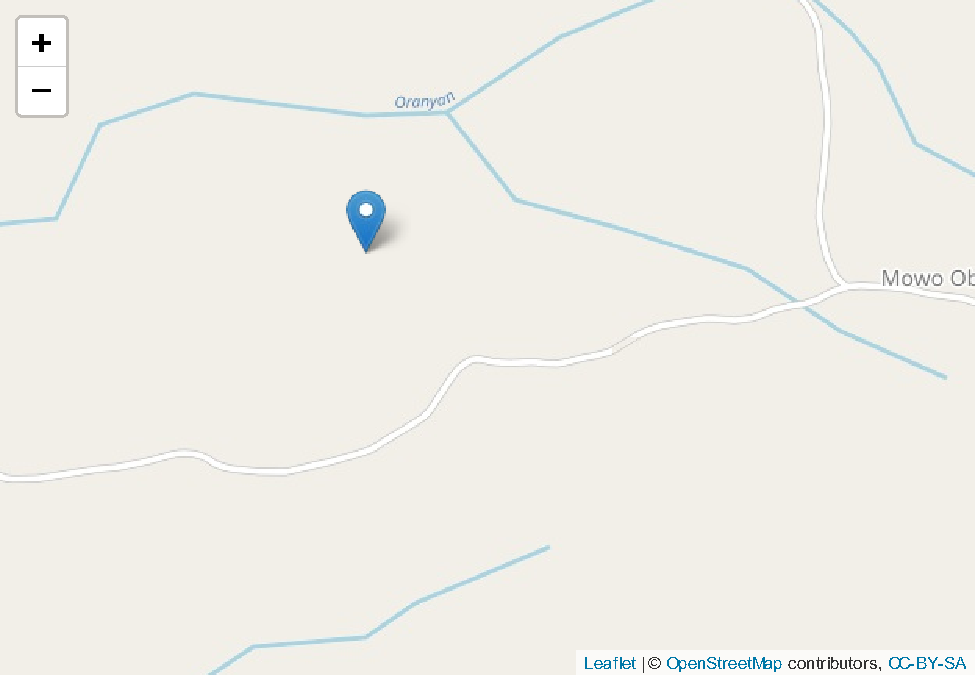
\includegraphics{Rticle-Template_files/figure-latex/Map-1.pdf} The
experiment was a factorial laid out in a RCBD with three replicates.

\hypertarget{statistical-analysis}{%
\section{Statistical analysis}\label{statistical-analysis}}

The data collected was analyzed using analysis of variance (ANOVA) and
significantly different means were seperated using Tukey's HSD at
(P\textless0.05).

\hypertarget{result}{%
\section{Result}\label{result}}

\begin{figure}
\centering
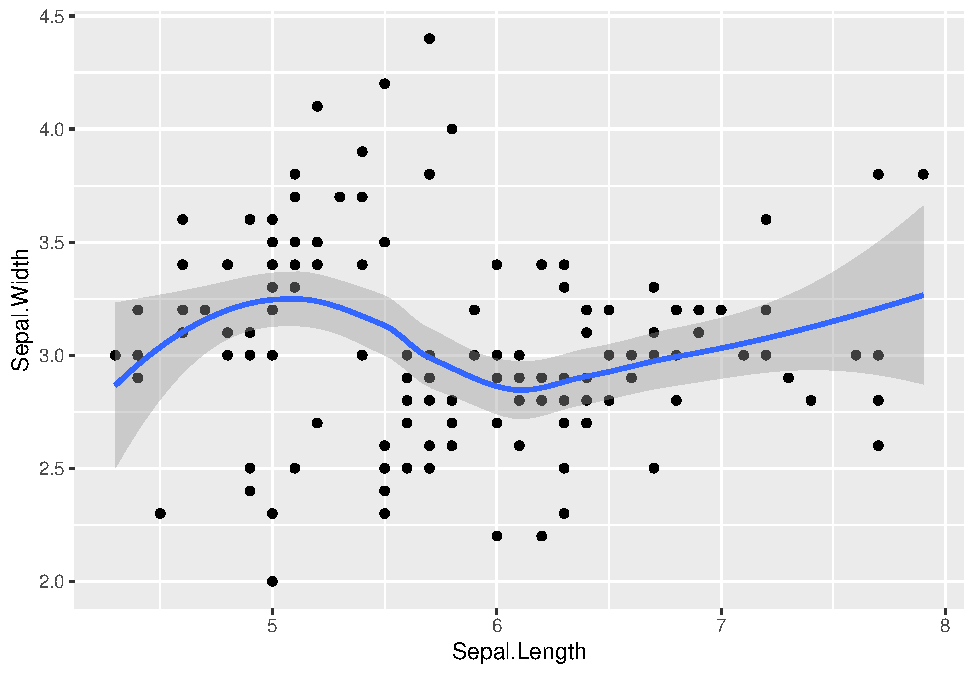
\includegraphics{Rticle-Template_files/figure-latex/unnamed-chunk-1-1.pdf}
\caption{plot1}
\end{figure}

\hypertarget{discussion}{%
\section{Discussion}\label{discussion}}

The traders were selling agricultural produce for the farmers. 50\% of
the traders were female, 30\% were teachers and 20\% were farmers which
shows that majority of the female living in the community were traders
(Table 1) \citep{adebayo2020assessment}.

According to plot1 the Sepal length has a strong negative relationship
with Sepal Width.

\hypertarget{conclusion}{%
\section{Conclusion}\label{conclusion}}

It is concluded that majority of the female traders focus more on
agricultural produce.

\hypertarget{acknowledgement}{%
\section{Acknowledgement}\label{acknowledgement}}

I am pleased to appreciate Prof Fatimah from University of Ibadan
Nigeria for assisting me throughout the computation of this manuscript.
I appreciate Dr Mr Femi for all hard work in encouraging me throughout
the research.

\renewcommand\refname{References}
\bibliography{mybibfile.bib}


\end{document}
